\documentclass[10pt, aspectratio=43]{beamer}

\usetheme{Berkeley}
% \usetheme[progressbar=frametitle]{metropolis}
\usepackage{appendixnumberbeamer}
\usepackage{listings}
\usepackage{proof}
\usepackage{biblatex}
\usepackage{xspace}
\newcommand{\themename}{\textbf{\textsc{metropolis}}\xspace}
\newcommand{\U}{\mathcal{U}}
\newcommand{\deq}{\equiv}
\newcommand{\Prod}[2]{\prod_{(#1)}{#2}}
\newcommand{\Sum}[2]{\sum_{(#1)}{#2}}
\newcommand{\0}{\mathbf{0}}
\newcommand{\1}{\mathbf{1}}
\newcommand{\2}{\mathbf{2}}
\newcommand{\N}{\mathbb{N}}
\newcommand{\Z}{\mathbb{Z}}
\newcommand{\Id}{\mathsf{Id}}
\newcommand{\refl}{\mathsf{refl}}
\newcommand{\Sph}{\mathbb{S}}

\newtheorem{axiom}{Axiom}
\setbeamertemplate{section page}{
  \begin{center}
    \vfill
    \begin{beamercolorbox}[sep=12pt,center]{section title}
      \usebeamerfont{section title}\insertsection
    \end{beamercolorbox}
    \vfill
  \end{center}
}
\AtBeginSection[]{
  \begin{frame}
    \sectionpage
  \end{frame}
}

\addbibresource{references.bib}

\title{A Brief Exposition to Type Theory}
\subtitle{(Bachelor's Thesis Presentation)}
\date{May 01, 2026}
\author{Naveen Maurya}
\institute{\SMALL Advisor: Prof. Siddhartha Gadgil \\ \vspace{0.1cm} \small Indian Institute of Science } 

\begin{document}

\maketitle

\begin{frame}{Table of contents}
  \setbeamertemplate{section in toc}[sections numbered]
  \tableofcontents%[hideallsubsections]
\end{frame}

\section{Foudational Systems} 
 
\subsection{What is a Foundational System?}

\begin{frame}{What is a Foundational System?}
    A foundational system is a framework that allows mathematicians to build mathematical objects and theories in.\\ 
    Zermelo-Frankel Set Theory is not complete by itself, since it lives in the language of \emph{first-order logic}.\\
    A \textbf{Foundational System} refers to both parts, the logical system and the infrastructure to express mathematical objects. \\
\end{frame}

\begin{frame}{What is a Foundational System?}
  Concretely, a Foundation System consists of
  \begin{itemize}
    \item A \textbf{Logical/Deductive system} specifying \emph{rules of inference} that dictate which inferences are
      allowed from existing context.
    \item An \textbf{Axiomatic system}, a schematic collection of \emph{axioms}, statements in the language of the deductive system,
      taken as true by assumption.
  \end{itemize}
  Usually in set-theoretic foundations, the former is \emph{first-order logic} and the latter is \emph{ZF or ZFC Set Theory}.
  Type Theory combines these two layers into the same framework.
\end{frame}

\section{Martin-L\"of Type Theory (MLTT)}

\subsection{A Description of MLTT}

\begin{frame}{(Intensional) Martin-L\"of Type Theory}
  \textbf{Some Basic Rules}
  \begin{itemize}
    \item Types are primitive objects.
    \item Type $A$ may be inhabited by a \emph{term/instance}, denoted $a : A$.
    \item A \emph{judgement} is an inference dervied from existing context by \emph{rules of inference}.
    \item Judements are either of the form:
      \begin{itemize}
      \item $a : A$ 
      \item $a \deq b : A$ or simply $a \deq b$
      \end{itemize}
    where `$\deq$' stands for \emph{judgemental equality}, an internal equality. 
    \item There is also \emph{propositional equality} denoted `$=$', a weaker notion corresonding to 
    equality as mathematical objects.
  \end{itemize}
\end{frame}

\begin{frame}{(Intensional) Martin-L\"of Type Theory} 
  \textbf{Logic in Type Theory}
  \begin{itemize}
    \item Types also function as logical objects, in particular, they can simulate propositions.
    \item A term $a : A$ where $A$ is a propositon is a \emph{proof} of $A$.
    \item Logic emerges through rules of inference given by Type Theory.
    \item Logical quantifiers such as $\land, \lor, \implies, \forall, \exists$ correspond to certain constructions over types.
    \item Type families $E : A \to U$ such that $E(a)$ are propositions for $a : A$ correspond to properties of terms of $A$.
    \item Type Theory's logic is constructive! 
   \end{itemize} 
\end{frame}

\begin{frame}{Universes}
  Type Theory postulates a chain of cumulative universes à la Russell:
  \[
    \U_0, \U_1, \U_2, \U_3, \ldots
  \]
  satisfying:
  \begin{itemize}
    \item $\U_i : \U_{i+1}$ for each $i$
    \item If $A : \U_i$, then $A : \U_{i+1}$
  \end{itemize}
  Each type is a term of some universe.
  Each universe is also a term of universes above it.
\end{frame}

\subsection{Inductive Types}

\begin{frame}{Inductive Types}
  There is a general schema for constructing new types, requiring:
  \begin{itemize}
    \item \textbf{Formation rules} to introduce an inductive type into context. 
    \item \textbf{Constructors/introduction rules} to introudce terms of the type.

    \item \textbf{Elimination rules} to consume terms of a type. \\
      (Usually by a \emph{recursion} or an \emph{induction} principle which define (dependent) functions on the type)

    \item \textbf{Computation rules} to specify action of elimination on the constructors.

  \end{itemize}
  These rules specify the behaviour of an inductive type by dictating the inference rules for the type 
  in the foundational system.
\end{frame}

\begin{frame}{Examples}
  \textbf{Natural Numbers Type ($\N$)}
  The natural numbers are an inductive type, given by the constructors 
  \begin{itemize}
    \item $\mathtt{zero} : \N$ 
    \item $\mathtt{succ} : \N \to \N$
  \end{itemize}
  To prove a property $E : \N \to \U$, it suffices to prove $E(\mathtt{zero})$ and for all $n : \N$, $E(n) \to E(\mathtt{succ}(n))$.

This is the usual \emph{principle of mathematical induction}!
\end{frame}

\begin{frame}{Type Formers}
  \renewcommand{\arraystretch}{1.2} % increase row height
  \setlength{\tabcolsep}{9pt}     % increase column spacing
  \centering
  \begin{tabular}{c  c  c}
  \hline
  \textbf{Type Former} & \textbf{Notation} & \textbf{Logical Analogue} \\
  \hline
  Function Type             & $A \to B$            & $A \implies B$ \\
  Dependent Function Type   & $\Prod{x:A}{B(x)}$ & $\forall x \in A, B(x)$ \\
  Dependent Pair Type       & $\Sum{x:A}{B(x)}$  & $\exists x \in A, B(x)$ \\
  Product Type              & $A \times B$            & $A \land B$ \\
  Coproduct Type            & $\0$               & $A \lor B$ \\
  Empty Type                & $\0$               & $\mathtt{False}$ \\
  Unit Type                 & $\1$               & $\mathtt{True}$ \\
  \hline
  \end{tabular}
\end{frame}

\subsection{Identity Types}

\begin{frame}{Identity Types}
  \begin{itemize}
    \item Equalities are encoded as an inductive type.
    \item For any $A : \U$ and $x, y : A$, proofs of equality $x = y$ are terms of $\Id_A(x,y)$. (Also denoted $x =_A y$)
    \item There is a construtor $\refl_a : a =_A a$.
    \item But one can now treat $(x =_A y)$ as a mathematical object to predicate over.
    \item One can have multiple, nonequivalent proofs of equality.
    \item Can have iterated identity types $\Id_{\Id(x,y)}(p,q)$ etc. 
    \item Bookeeeping these nonequivalences ad infinitum captures structure. 
  \end{itemize}
  \pause
  \textbf{Remark.}
  An equality $p : A =_\U B$ in a universe gives a transport $p_* : E(A) \to E(B)$ for any $E : A \to \U$.
\end{frame}

\section{Homotopy Type Theory}

\begin{frame}{(Weak) $\infty$-Groupoid}
  A (weak) $\infty$-groupoid is a collection of:
  \begin{itemize}
    \item $0$-cells called points
    \item $1$-cells between two points
    \item \ldots
    \item $(n+1)$-cells between two $n$-cells
  \end{itemize}
  following
  \begin{itemize}
    \item Concatenation and identity leading to associativity and unit up to higher dimensional cells. 
    \item All $(n+1)$ cells being invertible up to $(n+2)$ cells.
  \end{itemize}
\end{frame}
%
%
% \begin{frame}{(Weak) $\infty$-Groupoid}
%   A (weak) $\infty$-groupoid is a collection of:
%   \begin{itemize}
%     \item Points, also called $0$-cells.
%     \item $(n + 1)$-cells for each $n \in \N$, each of which lies between two $n$-cells, denoted $p : x \to y$
%     \item For $n$-cells, a composition $\circ$, given $p : x \to y$ and $q : y \to z$, giving $q \circ p : x \to z$
%     \item For $n$-cell $x$, an $(n+1)$ cell $1_x : x \to x$.
%     \item (Associativity) For $(n + 1)$-cells $p : x \to y, q : y \to z, r : z \to w$, an $(n+2)$ cell,
%       $\alpha_{pqr} : (r \circ q) \circ p \to r \circ (q \circ p)$. 
%     \item (Unit) For $n$-cell $x$ and $(n+1)$ cell $p : x \to y$, $(n+2)$-cells $\mu : 1_y \circ p \to  p$ and $\eta : p \circ 1_x = p$. 
%     \item (Inverese) For $(n+1)$ cell $p : x \to y$, an $(n+1)$ cell $p^{-1} : y \to x$, and a $(n+2)$-cell
%       $\lambda_p : p \circ p^{-1} \to 1_y$, and $\rho_p : p^{-1} \circ p \to 1_x$.
%   \end{itemize}
%   adsfaf
% \end{frame}
%
\subsection{The Homotopy Interpretation}

\begin{frame}{The Homotopy Interpretation} 
  In HoTT, types in HoTT can be interpreted as either:
  \begin{itemize}
    \item topological spaces upto weak homotopy equivalence, 
    \item (weak) $\infty$-groupoids from higher dimensional category theory. 
  \end{itemize}
  One can establish an equivalence between these interpretations via the \emph{Homotopy Hypothesis}. 
  \begin{block}{Homotopy Hypothesis (Grothendieck)}
   A space $X$ is determined upto weak homotopy equivalence by its fundamental groupoid $\Pi_\infty (X)$. 
  \end{block}
\end{frame}

\begin{frame}{Identity Types as Path Spaces}
  
  Identity Types have a homotopical intepretation in HoTT: 
  \centering
\vspace{1em}

\begin{overlayarea}{\textwidth}{5cm} % reserve space
    \only<1>{
      \centering
    {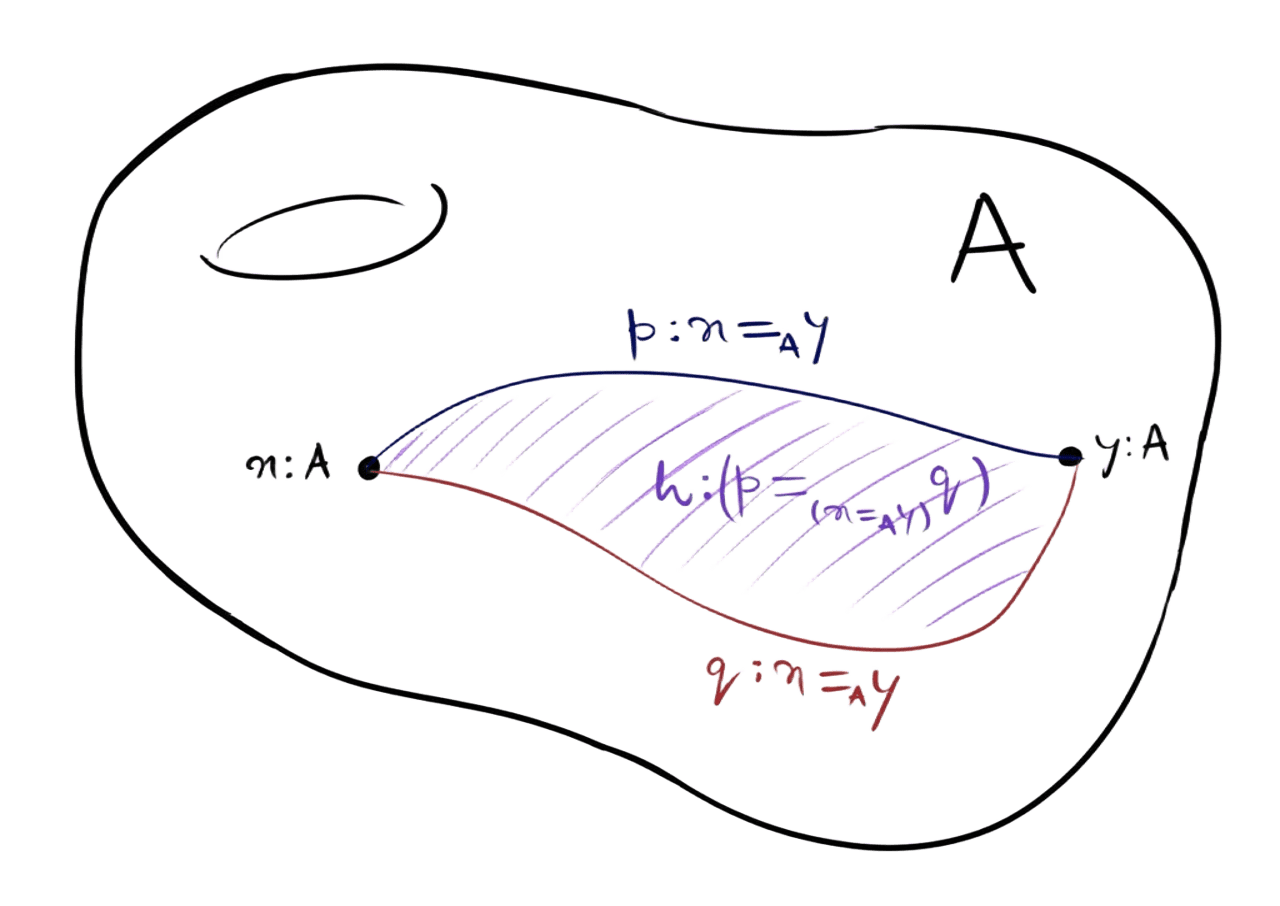
\includegraphics[width=0.8\textwidth]{figures/homotopy_correct.png}}
    }
    \only<2>{
        \begin{block}{}
            \begin{align*}
\text{Types} \qquad \leftrightarrow& \qquad \text{Spaces} \\
 \text{Terms } x : A \qquad \leftrightarrow& \qquad \text{Points } x \text{ of } A \\
  p : \Id_A(x,y) \qquad \leftrightarrow&  \qquad \text{Paths from } x \text{ to } y \\ 
 h : \Id_{\Id_A(x,y)}(p,q) \qquad \leftrightarrow& \qquad \text{Homotopies between} \\
                                & \qquad \text{parallel paths } p, q : x =_A y \\
                         \ldots \qquad \leftrightarrow & \qquad \ldots
  \end{align*}
        \end{block}
    }
\end{overlayarea}
\end{frame}

\subsection{The Univalence Axiom}

\begin{frame}{The Univalence Axiom}
  \only<2-3>{
    Consider the groups
    \begin{align*}
      (\Z / 2 \Z, +) \qquad \text{ and } \qquad (\{\pm 1\}, \cdot)
    \end{align*}
  Obviously isomorphic, so must share properties and theorems proven in group theory. \\
  \pause
  But no obvious way to translate theorems from one to another!
 
  }
 \only<4->{
  In practice, mathematicians tend to informally identify isomorphic objects, and extend properties by abuse of notation.\\ 
  To capture this formally, Voevodsky proposed the Univalence axiom:
  \begin{axiom}[Univalence]
    Let $A, B : \mathcal{U}$, then we have an equivalence
    \[ (A \simeq B) \simeq (A =_{\mathcal{U}} B)\]
  \end{axiom}
  \pause
  \begin{itemize}
    \item Given equivalent types, one may transport theorems and proofs along the path provided by univalence!
    \item Univalence formalizes this mathematical practice.
  \end{itemize}
} 
\end{frame}

\section{Limitations}

\subsection{Limitations of HoTT}
\begin{frame}{Limitations of HoTT}
  Despite providing a strong interpretive shift, HoTT fails to be completely satisfactory due to the following
  \begin{itemize}
    \item Lacks good computational properties 
    \item Univalence is an axiom, so is computationally troublesome
    \item \emph{Computational canonicity} and \emph{normalization} are not known to hold
  \end{itemize}
  \pause
  Alternatives such as \textbf{Cubical Type Theory} are partially satisfactory but further work is needed.
\end{frame}

\begin{frame}{References}
    % This command prints the bibliography
    \printbibliography

    % Use \nocite{*} if you want to include ALL entries from the .bib file,
    % even those you didn't cite with \cite{} in the main text.
    \nocite{*}
\end{frame}

\begin{frame}
    \begin{center}
        \Huge{Questions?}
    \end{center}
\end{frame}
\end{document}
